\input cwebmac

% piruett
%\input graphicx.tex
\input miniltx
\input graphicx

\nocon % omit table of contents
\datethis % print date on listing


\N{1}{1}Introduction. This is the firmware portion of the propulsion system for
our
Champbot.
It features separate thrust and steering as well as piruett turning.

This will facilitate motion by taking ``thrust'' and ``radius'' pulse-width,
or PWC, inputs from the Futaba-Kyosho RC receiver and converting them to the
appropriate motor actions.
Thrust is Channel 2, entering analog input A1, and Radius is channel 1, at A0.
The action will be similar to driving an RC car or boat.
By keeping it natural, it should be easier to navigate the course than with a
skid-steer style control.

We are using the Wingxing DBH-01C.
The Inputs are unique on this as the PWM logic input is a two bit value at IN1
and IN2. Values 0 and 3 are logic LOW.

The example in the datasheet has PWM on IN1 and LOW on IN2 for forward.
For reverse, LOW on IN1 and PWM on IN2.
We don't want PWM hopping between pins so we keep PWM on IN1.
The result of this mode is that PWM as IN1 is inverted when IN2 is HIGH.
This means we need to flip the PWM when the direction pin goes HIGH.

The larboard motor PWM word will be available at Pins 3 and 5.
The starboard motor PWM word will be at 4 and 6.
OC0A and OC0B is on pins 5 and 6  (D8 and D6) and are the PWM.
A fail-safe relay output will be at pin 8.

\fi

\N{1}{2}Implementation.
The Futaba receiver has two PWC channels.
The pulse-width from the receiver is at 20~ms intervals.
The on-time ranges from 1000--2000~$\mu$s including trim.
1500~$\mu$s is the pulse-width for stop.
The levers cover $\pm$400~$\mu$s and the trim covers the last 100~$\mu$s.

The median time will be subtracted from them for a pair of signed values
thrust and radius. The value will be scaled.

The thrust and radius will be translated to power to the
port and starboard motors.
When near median the motors will be disabled through a dead-band.
Stiction in the motor probably wouldn't allow it to move anyway, at this low
duty-cycle. Both the PWM and safety relay will open.
The motors will also be disabled when there are no input pulses; in this way
champ wont run-off if the range is exceeded. This function is handled by the
watchdog timer.

The radius control will also be the rotate control, if thrust is zero.
Timer-Counter 0 is used for the PWM.

The ATmega328 has a 16 bit PWMs with two comparators, Timer 1.
This has an ``Input Capture Unit'' that may be used for PWC decoding.
PWC being the type of signal from the RC receiver.
That seems like as elegant a solution as I will find and it is recommended by
Atmel to use it for this purpose.

The best way to use this nice feature is to
take the PWC signals into the MUX, through the comparator and into the Input
Capture Unit.

For the PWC measurement, this app note, AVR135, is helpful:
www.atmel.com/images/doc8014.pdf


In the datasheet, this section is helpful: 16.6.3

An interesting thing about this Futaba receiver is that the pulses are in
series.
The channel two's pulse is first, followed the channel one.
In fact, channel two's fall is perfectly aligned with channel one's rise.
This means that it will be possible to capture all of the pulses.

After the two pulses are captured, there's an 18~ms dead-time before the next
round. That's over 250,000 clock cycles.
This will provide ample time to do math and set the motor PWMs.


Extensive use was made of the datasheet, Atmel
``Atmel-8271I-AVR- ATmega-Datasheet\_10/2014''.


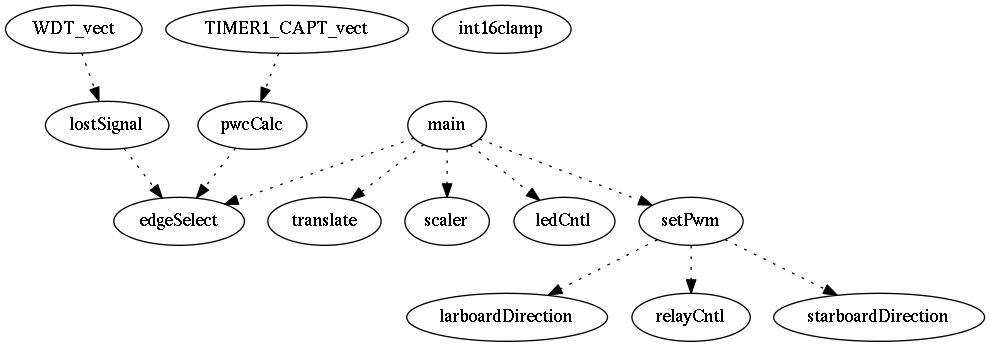
\includegraphics[width=35 pc]{piruett.png}

I originaly wanted to use the word "Port" for the left-hand side, when facing
the front. On a microcontroller that name is used for all of the ports so I
chose the older word ``larboard''.

\Y\B\X6:Include\X\6
\X7:Types\X\6
\X9:Prototypes\X\6
\X10:Global variables\X\par
\fi

\M{3}\PB{\.{"F\_CPU"}} is used to convey the Trinket Pro clock rate.
\Y\B\4\D$\.{F\_CPU}$ \5
\T{16000000\$U\$L}\par
\fi

\M{4}Here are some Boolean definitions that are used.
\Y\B\4\D$\.{ON}$ \5
\T{1}\par
\B\4\D$\.{OFF}$ \5
\T{0}\par
\B\4\D$\.{SET}$ \5
\T{1}\par
\B\4\D$\.{CLEAR}$ \5
\T{0}\par
\B\4\D$\.{TRUE}$ \5
\T{1}\par
\B\4\D$\.{FALSE}$ \5
\T{0}\par
\B\4\D$\.{FORWARD}$ \5
\T{1}\par
\B\4\D$\.{REVERSE}$ \5
\T{0}\par
\B\4\D$\.{CLOSED}$ \5
\T{1}\par
\B\4\D$\.{OPEN}$ \5
\T{0}\par
\B\4\D$\.{STOPPED}$ \5
\T{0}\par
\fi

\M{5}Here are some other definitions.
\Y\B\4\D$\.{CH2RISE}$ \5
\T{0}\par
\B\4\D$\.{CH2FALL}$ \5
\T{1}\par
\B\4\D$\.{CH1FALL}$ \5
\T{2}\par
\B\4\D$\.{MAX\_DUTYCYCLE}$ \5
\T{98}\SHC{ 98\% to support charge pump of bridge-driver }\par
\fi

\M{6}\B\X6:Include\X${}\E{}$\6
\8\#\&{include} \.{<avr/io.h>}\SHC{ need some port access }\6
\8\#\&{include} \.{<avr/interrupt.h>}\SHC{ have need of an interrupt }\6
\8\#\&{include} \.{<avr/sleep.h>}\SHC{ have need of sleep }\6
\8\#\&{include} \.{<avr/wdt.h>}\SHC{ have need of watchdog }\6
\8\#\&{include} \.{<stdlib.h>}\6
\8\#\&{include} \.{<stdint.h>}\par
\U2.\fi

\M{7}Here is a structure type to keep track of the state of remote-control
input, e.g. servo timing. Rise and Fall indicate the PWC edges.
\PB{\.{"edge"}} is set to the edge type expected for the interrupt.

\Y\B\4\X7:Types\X${}\E{}$\6
\&{typedef} \&{struct} ${}\{{}$\1\6
\\{uint16\_t}\\{ch2rise};\6
\\{uint16\_t}\\{ch2fall};\6
\\{uint16\_t}\\{ch1fall};\6
\\{uint16\_t}\\{ch1duration};\6
\\{uint16\_t}\\{ch2duration};\6
\\{uint8\_t}\\{edge};\6
\\{uint8\_t}\\{lostSignal};\7
\&{const} \\{uint16\_t}\\{minIn};\SHC{ input, minimum }\6
\&{const} \\{uint16\_t}\\{maxIn};\SHC{ input, maximum }\2\6
${}\}{}$ \&{inputStruct};\par
\A8.
\U2.\fi

\M{8}Here is a structure type to keep track of the state of translation items.
\Y\B\4\X7:Types\X${}\mathrel+\E{}$\6
\&{typedef} \&{struct} ${}\{{}$\1\6
\\{int16\_t}\\{thrust};\SHC{ -255 to 255 }\6
\\{int16\_t}\\{radius};\SHC{ -255 to 255 }\6
\\{int16\_t}\\{track};\SHC{    1 to 255 }\6
\\{int16\_t}\\{starboardOut};\SHC{ -255 to 255 }\6
\\{int16\_t}\\{larboardOut};\SHC{ -255 to 255 }\7
\&{const} \\{int16\_t}\\{minOut};\SHC{ output, minimum }\6
\&{const} \\{int16\_t}\\{maxOut};\SHC{ output, maximum }\6
\&{const} \\{int8\_t}\\{deadBand};\SHC{ width of zero in terms of output units
}\2\6
${}\}{}$ \&{transStruct};\par
\fi

\M{9}\B\X9:Prototypes\X${}\E{}$\6
\&{void} \\{relayCntl}(\\{int8\_t}\\{state});\6
\&{void} \\{ledCntl}(\\{int8\_t}\\{state});\6
\&{void} \\{larboardDirection}(\\{int8\_t}\\{state});\6
\&{void} \\{starboardDirection}(\\{int8\_t}\\{state});\6
\&{void} \\{pwcCalc}(\&{inputStruct} ${}{*});{}$\6
\&{void} \\{edgeSelect}(\&{inputStruct} ${}{*});{}$\7
\\{int16\_t}\\{scaler}(\&{inputStruct} ${}{*},\39{}$\&{transStruct} ${}{*},\39%
\\{uint16\_t}\\{input});{}$\7
\&{void} \\{translate}(\&{transStruct} ${}{*});{}$\6
\&{void} \\{setPwm}(\&{transStruct} ${}{*});{}$\6
\&{void} \\{lostSignal}(\&{inputStruct} ${}{*}){}$;\par
\U2.\fi

\M{10}
My lone global variable is a function pointer.
This lets me pass arguments to the actual interrupt handlers.
This pointer gets the appropriate function attached by the \PB{\.{"ISR()"}}
function.

This input structure is to contain all of the external inputs.

\Y\B\4\X10:Global variables\X${}\E{}$\6
$\&{void}({*}\\{handleIrq}){}$(\&{inputStruct} ${}{*})\K\NULL{}$;\7
\&{int} \\{main}(\&{void})\1\1\7
$\{{}$\Y\par
\U2.\fi

\M{11}
The Futaba receiver leads with channel two, rising edge, so we will start
looking for that by setting \PB{\.{"edge"}} to look for a rise on channel 2.

Center position of the controller results in a count of about 21250,
hard left, or up, with trim reports about 29100 and hard right, or down,
with trim reports about 13400.

About 4/5ths of that range are the full swing of the stick, without trim.
This is from about 14970 and 27530 ticks.

\PB{\.{".minIn"}} \PB{\.{".maxIn"}} are the endpoints of the normal stick
travel.
The units are raw counnts as the Input Capture Register will use.

At some point a calibration feature could be added which could populate these
but the numbers here were from trial and error and seem good.

Until we have collected the edges we will assume there is no signal.
\Y\B\&{inputStruct} \\{input\_s} $\K$ $\{$ $.$ $\\{edge}\K\.{CH2RISE}$ $,$ $.$
$\\{minIn}\K\T{14970}$ $,$ $.$ $\\{maxIn}\K\T{27530}$ $,$ $.$ $\\{lostSignal}\K%
\.{TRUE}$ $\}$  ;\par
\fi

\M{12}
This is the structure that holds output parameters.
It's instantiated with the endpoint constants.
\Y\B\&{transStruct} \\{translation\_s} $\K$ $\{$ $.$ $\\{minOut}\K{-}\T{255}$
$,$ $.$ $\\{maxOut}\K\T{255}$ $,$ $.$ $\\{deadBand}\K\T{10}$ $\}$  ;\par
\fi

\M{13}
Here the interrupts are disabled so that configuring them doesn't set it off.
\Y\B\\{cli}(\,);\7
\X45:Initialize the inputs and capture mode\X\X42:Initialize pin outputs\X%
\X47:Initialize watchdog timer\X\Y\par
\fi

\M{14}
Any interrupt function requires that bit ``Global Interrupt Enable''
is set; usually done through calling \PB{\.{"sei()"}}.
\Y\B\\{sei}(\,);\Y\par
\fi

\M{15}

The PWM is used to control larboard and starboard motors through OC0A (D5) and
OC0B (D6), respectivly.
\Y\B\X49:Initialize the Timer Counter 0 for PWM\X\par
\fi

\M{16}
Rather than burning loops, waiting the ballance of 18~ms for something to
happen, the \PB{\.{"sleep"}} mode is used.
The specific type of sleep is \PB{\.{"idle"}}.
In idle, execution stops but timers, like the Input Capture Unit and PWM
continue to operate.
Interrupts, either \PB{\\{Input}\\{Capture}} or \PB{\\{Watchdog}},  are used to
wake it up.

It's important to note that an ISR procedure must be defined to allow the
program to step past the sleep statement, even if it is empty.
This stumped me for a good while.
\Y\B\X43:Configure to idle on sleep\X\7
\\{ledCntl}(\.{OFF});\par
\fi

\M{17}
Since \PB{\.{"edge"}} is already set, calling \PB{\\{edgeSelect}(\,)} will get
it ready for
the first rising edge of channel~2.
Subsequent calls to \PB{\\{edgeSelect}} rotates it to the next edge type.
\Y\B$\\{edgeSelect}({\AND}\\{input\_s}){}$;\par
\fi

\M{18}
This is the loop that does the work.
It should spend most of its time in ``sleep\_mode'', comming out at each
interrupt event caused by an edge or watchdog timeout.
\Y\B\&{for} ( ;  ; \,) $\{{}$\Y\par
\fi

\M{19}
Now that a loop is started, the PWM is value and we wait in
\PB{\.{"idle"}} for the edge on the channel selected. Each sucessive loop will
finish
in the same way.
After three passes \PB{\.{"translation\_s"}} will have good values.

\Y\B$\\{setPwm}({\AND}\\{translation\_s});{}$\6
\\{sleep\_mode}(\,);\par
\fi

\M{20}
If execution arrives here, some interrupt has woken it from sleep and some
vector has possibly run. The possibility is first checked.
The pointer \PB{\.{"handleIrq"}} will be assigned the value of the responsible
function and then executed.
After that the IRQ is nulled so as to avoid repeating the action, should it
wake for some other reason.


\Y\B\&{if} ${}(\\{handleIrq}\I\NULL){}$\5
${}\{{}$\1\7
${}\\{handleIrq}({\AND}\\{input\_s});{}$\6
${}\\{handleIrq}\K\NULL;{}$\6
\4${}\}{}$\2\6
${}\\{translation\_s}.\\{radius}\K\\{scaler}({\AND}\\{input\_s},\39{\AND}%
\\{translation\_s},\39\\{input\_s}.\\{ch1duration});{}$\6
${}\\{translation\_s}.\\{thrust}\K\\{scaler}({\AND}\\{input\_s},\39{\AND}%
\\{translation\_s},\39\\{input\_s}.\\{ch2duration});{}$\6
${}\\{translation\_s}.\\{track}\K\T{100}{}$;\C{ represent unit-less
prop-to-prop distance }\6
${}\\{translate}({\AND}\\{translation\_s}){}$;\par
\fi

\M{21}
The LED is used to indicate PWM zeros.
\Y\B\&{if} ${}(\\{translation\_s}.\\{larboardOut}\V\\{translation\_s}.%
\\{starboardOut}){}$\1\5
\\{ledCntl}(\.{OFF});\2\6
\&{else}\1\5
\\{ledCntl}(\.{ON});\2\7
$\}{}$\C{ end for }\7
\&{return} \T{0};\7
$\}{}$\C{ end main() }\par
\fi

\N{1}{22}Supporting routines, functions, procedures and configuration
blocks.


\fi

\M{23}
Here is the ISR that fires at each captured edge.
Escentialy it grabs and processes the \PB{\\{Input}\\{Capture}} data.
\Y\B\.{ISR}(\\{TIMER1\_CAPT\_vect})\7
${}\{{}$\1\7
${}\\{handleIrq}\K{\AND}\\{pwcCalc}{}$;\7
\4${}\}{}$\2\Y\par
\fi

\M{24}
This is a variant of \PB{\\{pwcCalc}} that only flips the \PB{\\{lostSignal}}
flag.
\Y\B\.{ISR}(\\{WDT\_vect})\7
${}\{{}$\1\7
${}\\{handleIrq}\K{\AND}\\{lostSignal}{}$;\7
\4${}\}{}$\2\Y\par
\fi

\M{25}
This procedure computes the durations from the PWC signal edge capture values
from the Input Capture Unit.
With the levers centered the durations should be about 1500~$\mu$s so at
16~Mhz the count should be near 24000.
The range should be 17600 to 30400 for 12800 counts, well within the range
of the 64 kib of the 16 bit register..


\Y\B\&{void} \\{pwcCalc}(\&{inputStruct} ${}{*}\\{input\_s}{}$)\1\1\7
$\{{}$\Y\par
\fi

\M{26}
On the falling edges we can compute the durations using modulus subtraction
and then set the edge index for the next edge.
Channel 2 leads so that rise is first.

Arrival at the last case establishes that there was a signal and clears
the flag and resets the watchdog timer.
\Y\B\&{switch} ${}(\\{input\_s}\MG\\{edge}){}$\5
${}\{{}$\1\6
\4\&{case} \.{CH2RISE}:\5
${}\\{input\_s}\MG\\{ch2rise}\K\.{ICR1};{}$\6
${}\\{input\_s}\MG\\{edge}\K\.{CH2FALL};{}$\6
\&{break};\6
\4\&{case} \.{CH2FALL}:\5
${}\\{input\_s}\MG\\{ch2fall}\K\.{ICR1};{}$\6
${}\\{input\_s}\MG\\{ch2duration}\K\\{input\_s}\MG\\{ch2fall}-\\{input\_s}\MG%
\\{ch2rise};{}$\6
${}\\{input\_s}\MG\\{edge}\K\.{CH1FALL};{}$\6
\&{break};\6
\4\&{case} \.{CH1FALL}:\5
${}\\{input\_s}\MG\\{ch1fall}\K\.{ICR1};{}$\6
${}\\{input\_s}\MG\\{ch1duration}\K\\{input\_s}\MG\\{ch1fall}-\\{input\_s}\MG%
\\{ch2fall};{}$\6
${}\\{input\_s}\MG\\{edge}\K\.{CH2RISE};{}$\6
${}\\{input\_s}\MG\\{lostSignal}\K\.{FALSE};{}$\6
\\{wdt\_reset}(\,);\C{ watchdog timer is reset at each edge capture }\6
\4${}\hbox{\hskip 1in}\}{}$\2\6
\\{edgeSelect}(\\{input\_s});\7
$\}{}$\Y\par
\fi

\M{27}
This procedure sets output to zero in the event of a lost signal.
\Y\B\&{void} \\{lostSignal}(\&{inputStruct} ${}{*}\\{input\_s}{}$)\7
${}\{{}$\1\7
${}\\{input\_s}\MG\\{lostSignal}\K\.{TRUE};{}$\6
${}\\{input\_s}\MG\\{edge}\K\.{CH2RISE};{}$\6
\\{edgeSelect}(\\{input\_s});\7
\4${}\}{}$\2\Y\par
\fi

\M{28}

The procedure edgeSelect configures the \PB{\.{"Input\ Capture"}} unit to
capture on
the expected edge type.

\Y\B\&{void} \\{edgeSelect}(\&{inputStruct} ${}{*}\\{input\_s}{}$)\1\1\7
$\{{}$\7
\&{switch} ${}(\\{input\_s}\MG\\{edge}){}$\5
${}\{{}$\1\6
\4\&{case} \.{CH2RISE}:\C{ To wait for rising edge on servo-channel 2 }\6
${}\.{ADMUX}\MRL{{\OR}{\K}}(\T{1}\LL\.{MUX0}){}$;\C{ Set to mux channel 1 }\6
${}\.{TCCR1B}\MRL{{\OR}{\K}}(\T{1}\LL\.{ICES1}){}$;\C{ Rising edge (23.3.2) }\6
\&{break};\6
\4\&{case} \.{CH2FALL}:\5
${}\.{ADMUX}\MRL{{\OR}{\K}}(\T{1}\LL\.{MUX0}){}$;\C{ Set to mux channel 1 }\6
${}\.{TCCR1B}\MRL{\AND{\K}}\CM(\T{1}\LL\.{ICES1}){}$;\C{ Falling edge (23.3.2)
}\6
\&{break};\6
\4\&{case} \.{CH1FALL}:\5
${}\.{ADMUX}\MRL{\AND{\K}}\CM(\T{1}\LL\.{MUX0}){}$;\C{ Set to mux channel 0 }\6
${}\.{TCCR1B}\MRL{\AND{\K}}\CM(\T{1}\LL\.{ICES1}){}$;\C{ Falling edge (23.3.2)
}\6
\4${}\}{}$\2\par
\fi

\M{29}
Since the edge has been changed, the Input Capture Flag should be cleared.
It's odd but clearing it involves writing a one to it.
\Y\B$\.{TIFR1}\MRL{{\OR}{\K}}(\T{1}\LL\.{ICF1}){}$;\C{ (per 16.6.3) }\7
$\}{}$\Y\par
\fi

\M{30}
Here is a simple procedure to flip the LED on or off.
\Y\B\&{void} \\{ledCntl}(\\{int8\_t}\\{state})\7
${}\{{}$\1\7
${}\.{PORTB}\K\\{state}\?\.{PORTB}\OR(\T{1}\LL\.{PORTB5}):\.{PORTB}\AND\CM(%
\T{1}\LL\.{PORTB5}){}$;\7
\4${}\}{}$\2\Y\par
\fi

\M{31}
Here is a simple procedure to flip the Relay Closed or Open from pin \#8.
\Y\B\&{void} \\{relayCntl}(\\{int8\_t}\\{state})\7
${}\{{}$\1\7
${}\.{PORTB}\K\\{state}\?\.{PORTB}\OR(\T{1}\LL\.{PORTB0}):\.{PORTB}\AND\CM(%
\T{1}\LL\.{PORTB0}){}$;\7
\4${}\}{}$\2\Y\par
\fi

\M{32}
Here is a simple procedure to set thrust direction on the larboard motor.
It includes inverting PWM in support of the H-Bridge direction by binary value.
In forward, the PWM value is 2 for high and 3 for low.
In reverse, the PWM value is 1 for high and 0 for low.

\Y\B\&{void} \\{larboardDirection}(\\{int8\_t}\\{state})\7
${}\{{}$\1\7
\&{if} (\\{state})\5
${}\{{}$\1\6
${}\.{PORTD}\MRL{{\OR}{\K}}(\T{1}\LL\.{PORTD3});{}$\6
\4${}\}{}$\2\6
\&{else}\5
${}\{{}$\1\6
${}\.{PORTD}\MRL{\AND{\K}}\CM(\T{1}\LL\.{PORTD3});{}$\6
\4${}\}{}$\2\7
\4${}\}{}$\2\Y\par
\fi

\M{33}
Here is a simple procedure to set thrust direction on the starboard motor.
It includes inverting PWM in support of the H-Bridge direction by binary value.
In forward, the PWM value is 2 for high and 3 for low.
In reverse, the PWM value is 1 for high and 0 for low.
\Y\B\&{void} \\{starboardDirection}(\\{int8\_t}\\{state})\7
${}\{{}$\1\7
\&{if} (\\{state})\5
${}\{{}$\1\6
${}\.{PORTD}\MRL{{\OR}{\K}}(\T{1}\LL\.{PORTD4});{}$\6
\4${}\}{}$\2\6
\&{else}\5
${}\{{}$\1\6
${}\.{PORTD}\MRL{\AND{\K}}\CM(\T{1}\LL\.{PORTD4});{}$\6
\4${}\}{}$\2\7
\4${}\}{}$\2\Y\par
\fi

\M{34}

\fi

\M{35}
The scaler function takes an input, in time, from the Input Capture
Register and returns a value scaled by the parameters in structure
\PB{\.{"inputScale\_s"}}.
\Y\B\\{int16\_t}\\{scaler}(\&{inputStruct} ${}{*}\\{input\_s},\39{}$%
\&{transStruct} ${}{*}\\{trans\_s},\39\\{uint16\_t}\\{input}{}$)\1\1\7
$\{{}$\7
\\{uint16\_t}\\{solution};\par
\fi

\M{36}
First, we can solve for the obvious cases.
One is where there is no signal; when \PB{\.{"lostSignal"}} is \PB{\.{"TRUE"}}.
The other is where the input exceeds the range.
This can easily happen if the trim is shifted.
\Y\B\&{if} ${}(\\{input\_s}\MG\\{lostSignal}\E\.{TRUE}){}$\1\5
\&{return} \T{0};\2\6
\&{if} ${}(\\{input}>\\{input\_s}\MG\\{maxIn}){}$\1\5
\&{return} \\{trans\_s}${}\MG\\{maxOut};{}$\2\6
\&{if} ${}(\\{input}<\\{input\_s}\MG\\{minIn}){}$\1\5
\&{return} \\{trans\_s}${}\MG\\{minOut}{}$;\2\par
\fi

\M{37}
If it's not that simple, then compute the gain and offset and then continue in
the usual way.
This is not really an efficient method, recomputing gain and offset every time
but we are not in a rush and it makes it easier since, if something changes,
I don't have to manualy compute and enter these value.

The constant \PB{\.{"ampFact"}} amplifies it so I can take advantage of the
extra
bits for precision.

Dead-band is applied when it returns.
\Y\B\&{const} \\{int32\_t}\\{ampFact}${}\K\T{128\$L};{}$\7
${}\\{int32\_t}\\{gain}\K(\\{ampFact}*(\\{int32\_t})(\\{input\_s}\MG\\{maxIn}-%
\\{input\_s}\MG\\{minIn}))/(\\{int32\_t})(\\{trans\_s}\MG\\{maxOut}-\\{trans%
\_s}\MG\\{minOut});{}$\6
${}\\{int32\_t}\\{offset}\K((\\{ampFact}*(\\{int32\_t})\\{input\_s}\MG%
\\{minIn})/\\{gain})-(\\{int32\_t})\\{trans\_s}\MG\\{minOut};{}$\6
${}\\{solution}\K(\\{ampFact}*(\\{int32\_t})\\{input}/\\{gain})-\\{offset};{}$\6
\&{return} ${}(\\{abs}(\\{solution})>\\{trans\_s}\MG\\{deadBand})\?%
\\{solution}:\T{0}{}$;\7
$\}{}$\Y\par
\fi

\M{38}
We need a way to translate \PB{\.{"thrust"}} and \PB{\.{"radius"}} in order to
carve a
\PB{\.{"turn"}}. This procedure should do this but it's not going to be perfect
as
drag and slippage make thrust increase progressivly more than speed.
Since \PB{\\{speed}} is not known, we will use \PB{\\{thrust}}.
It should steer OK as long as the speed is constant and small changes in speed
should not be too disruptive.

The constant \PB{\.{"ampFact"}} amplifies it so I can take advantage of the
extra
bits.

This procedure is intended for values from -255 to 255.
\Y\B\&{void} \\{translate}(\&{transStruct} ${}{*}\\{trans\_s}{}$)\1\1\7
$\{{}$\7
$\\{int16\_t}\\{speed}\K\\{trans\_s}\MG\\{thrust}{}$;\C{ we are assuming it's
close }\6
\\{int16\_t}\\{rotation};\6
\\{int16\_t}\\{difference};\6
\\{int16\_t}\\{piruett};\7
\&{const} \\{int16\_t}\\{max}${}\K(\.{MAX\_DUTYCYCLE}*\.{UINT8\_MAX})/%
\T{100};{}$\6
\&{const} \\{int16\_t}\\{ampFact}${}\K\T{128}{}$;\par
\fi

\M{39}
Here we convert desired radius to thrust-difference by scaling to speed.
Then that difference is converted to rotation by scaling it with \PB{%
\.{"track"}}.
The radius sensitivity is adjusted by changing the value of \PB{\.{"track"}}.
\Y\B$\\{difference}\K(\\{speed}*((\\{ampFact}*\\{trans\_s}\MG\\{radius})/%
\.{UINT8\_MAX}))/\\{ampFact};{}$\6
${}\\{rotation}\K(\\{trans\_s}\MG\\{track}*((\\{ampFact}*\\{difference})/%
\.{UINT8\_MAX}))/\\{ampFact};{}$\6
${}\\{piruett}\K(((\\{ampFact}*\\{trans\_s}\MG\\{radius})/\.{UINT8\_MAX}))/%
\\{ampFact}{}$;\par
\fi

\M{40}
Any rotation involves one motor turning faster than the other.
At some point, faster is not possible and so the requiered clipping is here.

\PB{\.{"max"}} is set at to support the limit of the bridge-driver's
charge-pump.
\Y\B\&{if} ${}((\\{speed}-\\{rotation})\G\\{max}){}$\1\5
${}\\{trans\_s}\MG\\{larboardOut}\K\\{max};{}$\2\6
\&{else} \&{if} ${}((\\{speed}-\\{rotation})\Z{-}\\{max}){}$\1\5
${}\\{trans\_s}\MG\\{larboardOut}\K{-}\\{max};{}$\2\6
\&{else} \&{if} ${}(\\{trans\_s}\MG\\{thrust}\E\.{STOPPED}{}$)\C{ here we
switch to piruett mode }\1\6
${}\\{trans\_s}\MG\\{larboardOut}\K{-}\\{piruett};{}$\2\6
\&{else}\1\5
${}\\{trans\_s}\MG\\{larboardOut}\K\\{speed}-\\{rotation};{}$\2\6
\&{if} ${}((\\{speed}+\\{rotation})\G\\{max}){}$\1\5
${}\\{trans\_s}\MG\\{starboardOut}\K\\{max};{}$\2\6
\&{else} \&{if} ${}((\\{speed}+\\{rotation})\Z{-}\\{max}){}$\1\5
${}\\{trans\_s}\MG\\{starboardOut}\K{-}\\{max};{}$\2\6
\&{else} \&{if} ${}(\\{trans\_s}\MG\\{thrust}\E\.{STOPPED}){}$\1\5
${}\\{trans\_s}\MG\\{starboardOut}\K\\{piruett};{}$\2\6
\&{else}\1\5
${}\\{trans\_s}\MG\\{starboardOut}\K\\{speed}+\\{rotation}{}$;\2\7
$\}{}$\7
\&{void} \\{setPwm}(\&{transStruct} ${}{*}\\{trans\_s}{}$)\1\1\7
$\{{}$\7
\&{if} ${}(\\{trans\_s}\MG\\{larboardOut}\G\T{0}){}$\5
${}\{{}$\1\6
\\{larboardDirection}(\.{FORWARD});\6
${}\.{OCR0A}\K(\\{uint8\_t})\\{trans\_s}\MG\\{larboardOut};{}$\6
\4${}\}{}$\2\6
\&{else}\5
${}\{{}$\1\6
\\{larboardDirection}(\.{REVERSE});\6
${}\.{OCR0A}\K(\\{uint8\_t})\\{trans\_s}\MG\\{larboardOut};{}$\6
\4${}\}{}$\2\6
\&{if} ${}(\\{trans\_s}\MG\\{starboardOut}\G\T{0}){}$\5
${}\{{}$\1\6
\\{starboardDirection}(\.{FORWARD});\6
${}\.{OCR0B}\K(\\{uint8\_t})\\{trans\_s}\MG\\{starboardOut};{}$\6
\4${}\}{}$\2\6
\&{else}\5
${}\{{}$\1\6
\\{starboardDirection}(\.{REVERSE});\6
${}\.{OCR0B}\K(\\{uint8\_t})\\{trans\_s}\MG\\{starboardOut};{}$\6
\4${}\}{}$\2\par
\fi

\M{41}
We must see if the fail-safe relay needs to be closed.
\Y\B\&{if} ${}(\\{trans\_s}\MG\\{larboardOut}\V\\{trans\_s}\MG%
\\{starboardOut}){}$\1\5
\\{relayCntl}(\.{CLOSED});\2\6
\&{else}\1\5
\\{relayCntl}(\.{OPEN});\2\7
$\}{}$\Y\par
\fi

\M{42}\B\X42:Initialize pin outputs\X${}\E{}$\SHC{ set the led port direction;
This is pin \#17 }\6
$\.{DDRB}\MRL{{\OR}{\K}}(\T{1}\LL\.{DDB5}){}$;\SHC{ set the relay port
direction; This is pin \#8 }\6
${}\.{DDRB}\MRL{{\OR}{\K}}(\T{1}\LL\.{DDB0}){}$;\SHC{ 14.4.9 DDRD – The Port
D Data Direction Register }\SHC{ larboard and starboard pwm outputs }\6
${}\.{DDRD}\MRL{{\OR}{\K}}((\T{1}\LL\.{DDD5})\OR(\T{1}\LL\.{DDD6})){}$;\SHC{
Data direction to output (sec 14.3.3) }\SHC{ larboard and starboard direction
outputs }\6
${}\.{DDRD}\MRL{{\OR}{\K}}((\T{1}\LL\.{DDD3})\OR(\T{1}\LL\.{DDD4})){}$;\SHC{
Data direction to output (sec 14.3.3) }\par
\U13.\fi

\M{43}\B\X43:Configure to idle on sleep\X${}\E{}$\6
${}\{{}$\1\6
${}\.{SMCR}\MRL{\AND{\K}}\CM((\T{1}\LL\.{SM2})\OR(\T{1}\LL\.{SM1})\OR(\T{1}\LL%
\.{SM0}));{}$\6
\4${}\}{}$\2\par
\U16.\fi

\M{44}
To enable this interrupt, set the ACIE bit of register ACSR.
\fi

\M{45}\B\X45:Initialize the inputs and capture mode\X${}\E{}$\6
${}\{{}$\SHC{ ADCSRA – ADC Control and Status Register A }\1\6
${}\.{ADCSRA}\MRL{\AND{\K}}\CM(\T{1}\LL\.{ADEN}){}$;\SHC{ Conn the MUX to (-)
input of comparator (sec 23.2) }\SHC{ 23.3.1 ADCSRB – ADC Control and Status
Register B }\6
${}\.{ADCSRB}\MRL{{\OR}{\K}}(\T{1}\LL\.{ACME}){}$;\SHC{ Conn the MUX to (-)
input of comparator (sec 23.2) }\SHC{ 24.9.5 DIDR0 – Digital Input Disable
Register 0 }\6
${}\.{DIDR0}\MRL{{\OR}{\K}}((\T{1}\LL\.{AIN1D})\OR(\T{1}\LL\.{AIN0D})){}$;\SHC{
Disable digital inputs (sec 24.9.5) }\SHC{ 23.3.2 ACSR – Analog Comparator
Control and Status Register }\6
${}\.{ACSR}\MRL{{\OR}{\K}}(\T{1}\LL\.{ACBG}){}$;\SHC{ Connect + input to the
band-gap ref (sec 23.3.2) }\6
${}\.{ACSR}\MRL{{\OR}{\K}}(\T{1}\LL\.{ACIC}){}$;\SHC{ Enable input capture mode
(sec 23.3.2) }\6
${}\.{ACSR}\MRL{{\OR}{\K}}(\T{1}\LL\.{ACIS1}){}$;\SHC{ Set for both rising and
falling edge (sec 23.3.2) }\SHC{ 16.11.8 TIMSK1 – Timer/Counter1 Interrupt
Mask Register }\6
${}\.{TIMSK1}\MRL{{\OR}{\K}}(\T{1}\LL\.{ICIE1}){}$;\SHC{ Enable input capture
interrupt (sec 16.11.8) }\SHC{ 16.11.2 TCCR1B – Timer/Counter1 Control
Register B }\6
${}\.{TCCR1B}\MRL{{\OR}{\K}}(\T{1}\LL\.{ICNC1}){}$;\SHC{ Enable input capture
noise canceling (sec 16.11.2) }\6
${}\.{TCCR1B}\MRL{{\OR}{\K}}(\T{1}\LL\.{CS10}){}$;\SHC{ No Prescale. Just count
the main clock (sec 16.11.2) }\SHC{ 24.9.1 ADMUX – ADC Multiplexer Selection
Register }\6
${}\.{ADMUX}\MRL{\AND{\K}}\CM((\T{1}\LL\.{MUX2})\OR(\T{1}\LL\.{MUX1})\OR(\T{1}%
\LL\.{MUX0})){}$;\SHC{ Set to mux channel 0 }\6
\4${}\}{}$\2\par
\U13.\fi

\M{46}
See section 11.8 in the datasheet for details on the Watchdog Timer.
This is in the ``Interrupt Mode''.
\fi

\M{47}\B\X47:Initialize watchdog timer\X${}\E{}$\6
${}\{{}$\1\6
${}\.{WDTCSR}\MRL{{\OR}{\K}}(\T{1}\LL\.{WDCE})\OR(\T{1}\LL\.{WDE});{}$\6
${}\.{WDTCSR}\K(\T{1}\LL\.{WDIE})\OR(\T{1}\LL\.{WDP2}){}$;\SHC{ reset after
about 0.25 seconds }\6
\4${}\}{}$\2\par
\U13.\fi

\M{48}
PWM setup isn't too scary.
Timer Count 0 is configured for ``Phase Correct'' PWM which, according to the
datasheet, is preferred for motor control.
OC0A (port) and OC0B (starboard) are set to clear on a match which creates a
non-inverting PWM.
The prescaler is set to clk/8 and with a 16 MHz clock the $f$ is about 3922 Hz.
\fi

\M{49}\B\X49:Initialize the Timer Counter 0 for PWM\X${}\E{}$\6
${}\{{}$\SHC{ 15.9.1 TCCR0A – Timer/Counter Control Register A }\1\6
${}\.{TCCR0A}\MRL{{\OR}{\K}}(\T{1}\LL\.{WGM00}){}$;\SHC{ Phase correct, mode 1
of PWM (table 15-9) }\6
${}\.{TCCR0A}\MRL{{\OR}{\K}}(\T{1}\LL\.{COM0A1}){}$;\SHC{ Set/Clear on
Comparator A match (table 15-4) }\6
${}\.{TCCR0A}\MRL{{\OR}{\K}}(\T{1}\LL\.{COM0B1}){}$;\SHC{ Set/Clear on
Comparator B match (table 15-7) }\6
${}\.{TCCR0A}\MRL{{\OR}{\K}}(\T{1}\LL\.{COM0A0}){}$;\SHC{ Clear on Comparator A
match (table 15-4) }\6
${}\.{TCCR0A}\MRL{{\OR}{\K}}(\T{1}\LL\.{COM0B0}){}$;\SHC{ Clear on Comparator B
match (table 15-7) }\SHC{ 15.9.2 TCCR0B – Timer/Counter Control Register B }\6
${}\.{TCCR0B}\MRL{{\OR}{\K}}(\T{1}\LL\.{CS01}){}$;\SHC{ Prescaler set to clk/8
(table 15-9) }\6
\4${}\}{}$\2\par

\U15.\fi


\inx
\fin
\con
